\subsubsection{The \emph{real} implemenation}

Eventually some code was developed  that handles a virtual disk. This code and
some details about the file format are described in this section.

\paragraph{The File Format}
This section describes the binary file format used by the file system inside a
virtual disk. The file is separated into three major parts. The header, index
and the data section. Each of them is described below.

\begin{figure}[h!]
\centering
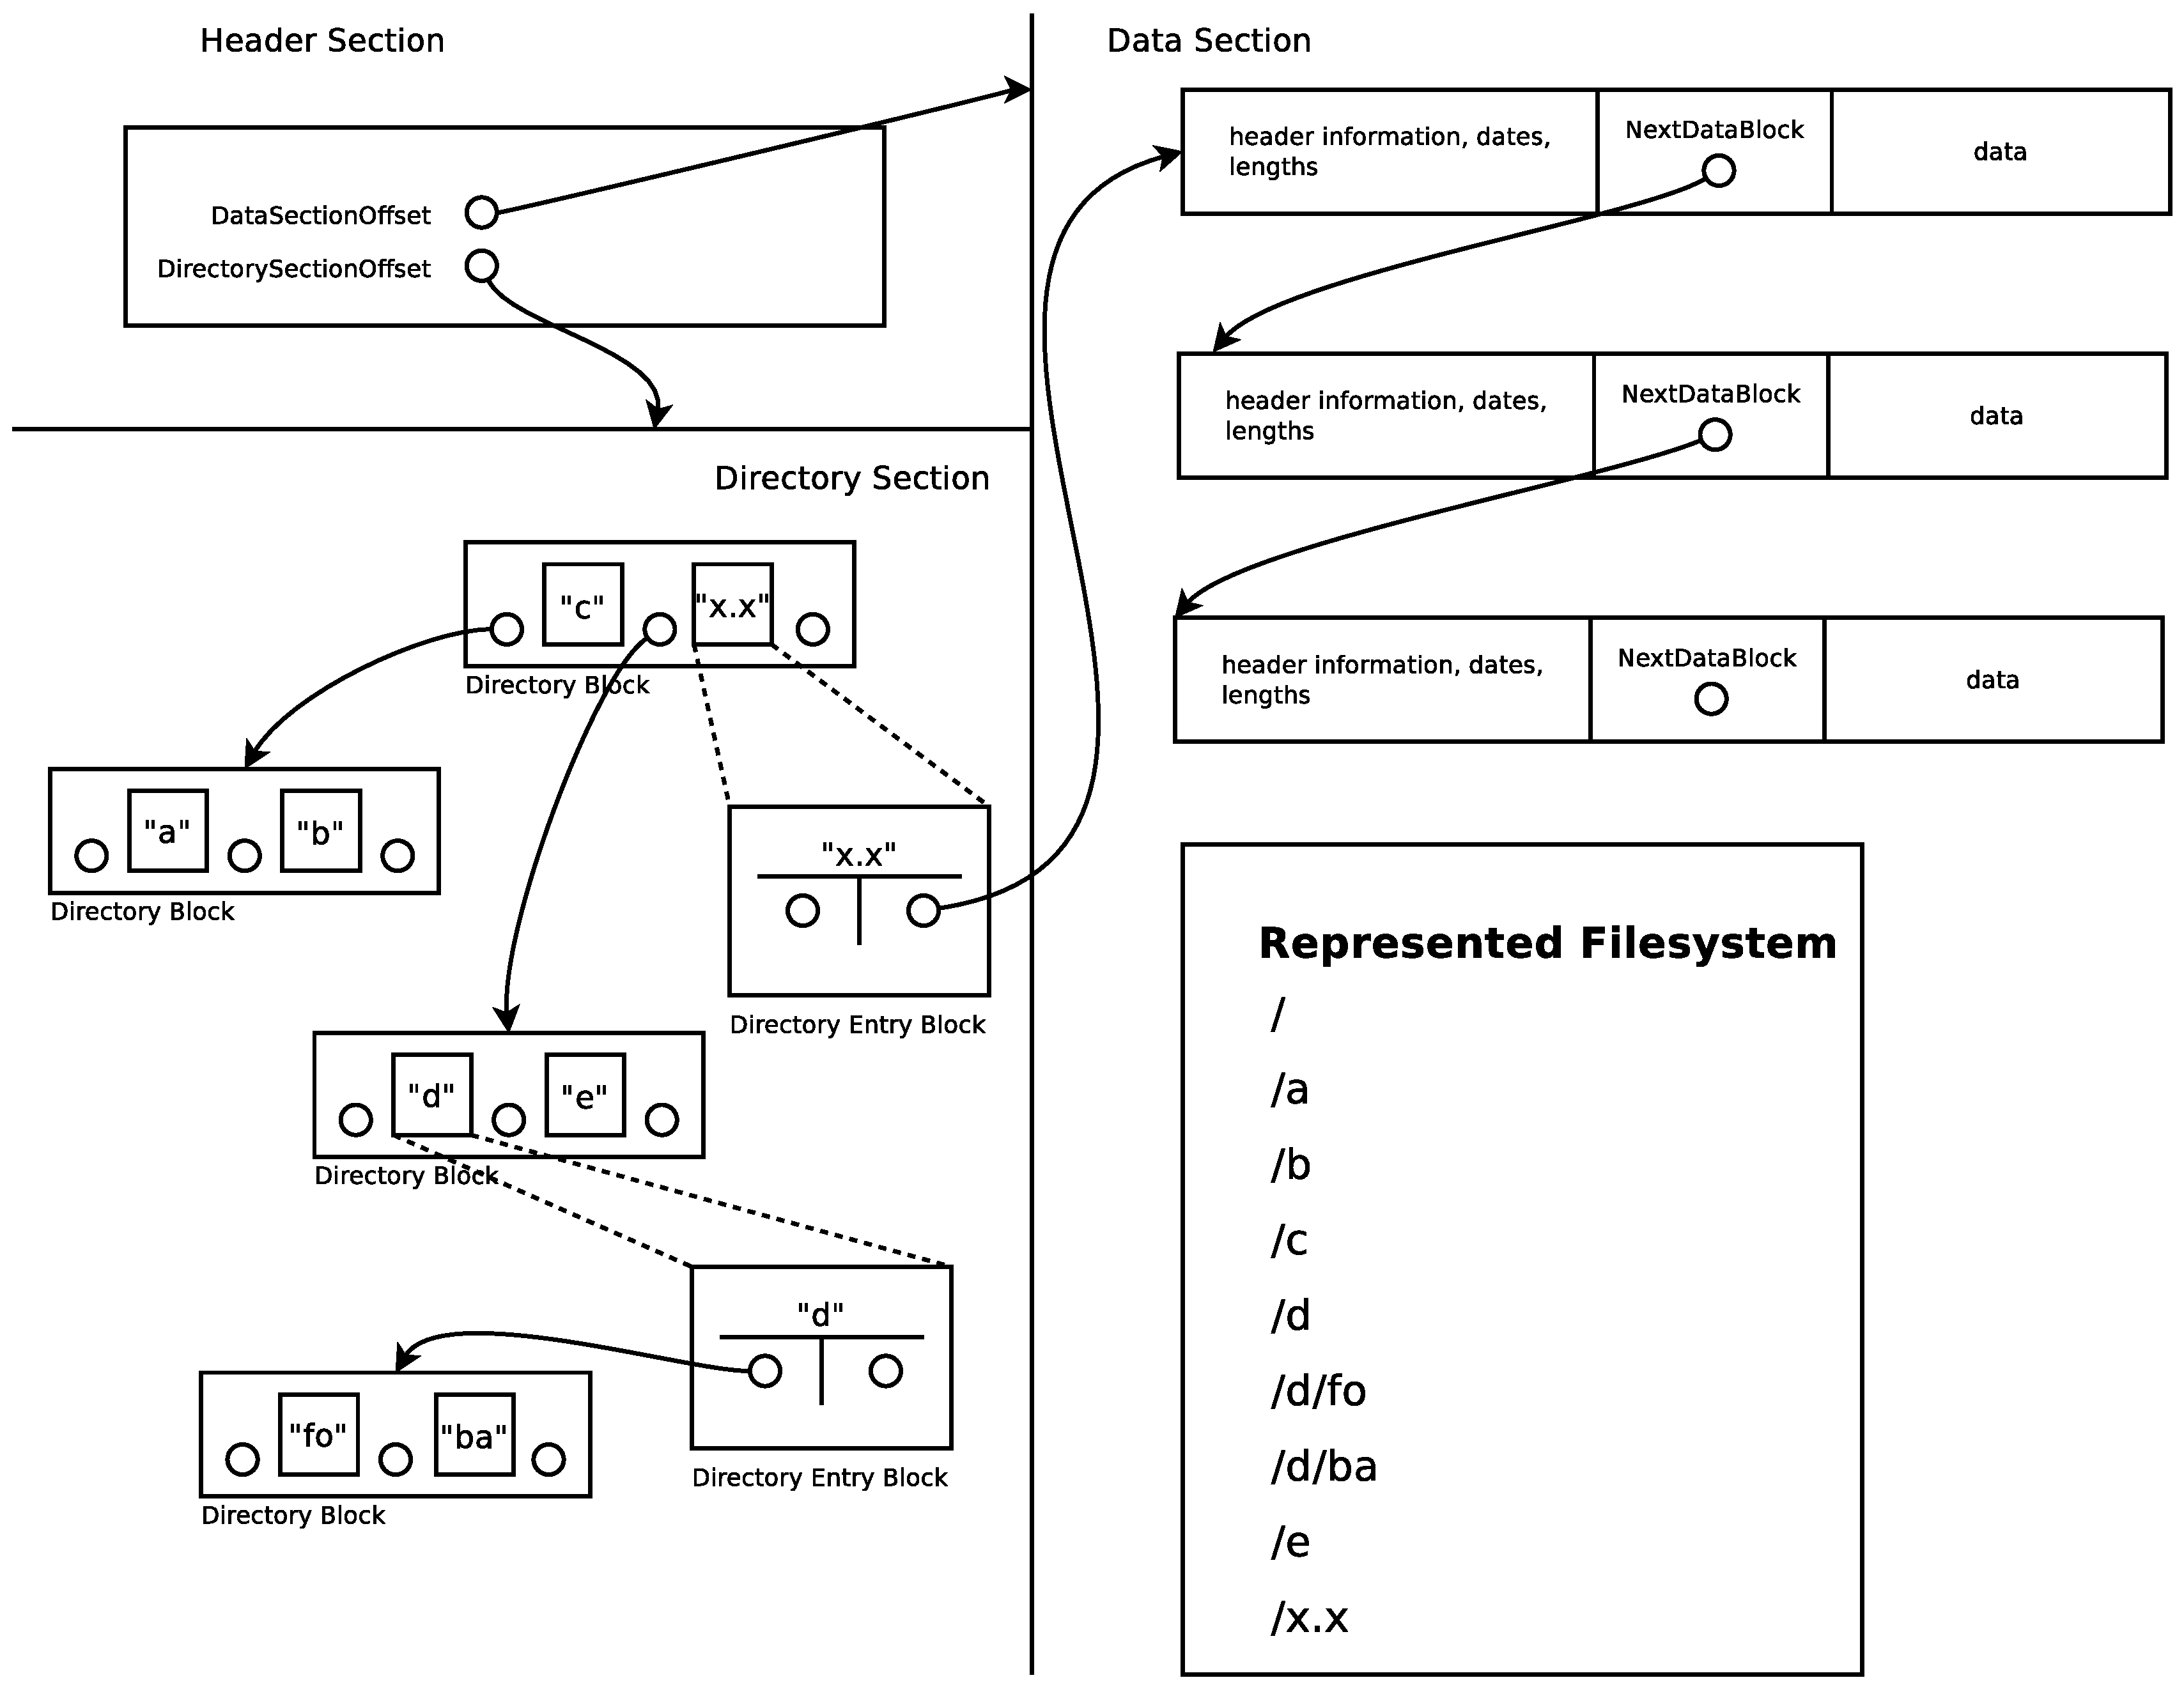
\includegraphics[width=1\textwidth]{figures/fileFormat.eps}
\caption{Overview of a disk}
\label{fig:disk_overview}
\end{figure}

\subparagraph{Header Section} The header section contains some general information
about the currently opened virtual disk. The details can be found in the
following table:

\begin{tabular}{|l|l|p{5cm}|}
\hline
  \textbf{Name} & \textbf{Length} & \textbf{Description}
\\  \hline
  Info & 50 byte UTF-8 String & Contains something like Badger VFS 2013 V1.0 
\\ \hline
  Version & 10 byte UTF-8 String & Contains something like "1.0"
\\ \hline
  Compression used & 20 byte UTF-8 String & null or indicates compression used for this file
\\ \hline
  Encryption used & 20 byte UTF-8 String & null or indicates encryption used for this file
\\ \hline
 DirectorySectionOffset & long (8 byte) &  File offset where the directory
 section starts \\ \hline
 DataSectionOffset & long (8 byte) &  File offset where our data section starts
\\ \hline
 SaltString & 8 bytes  & Salt used to hash username and password randomly string generated while creating this
   file
 \\ \hline
  Password & xxx bytes  & CryptoHash (SHA-whatever) of Password+SaltString
\\ \hline

\end{tabular}


\subparagraph{Directory Section}
The directory section describes which files and folders belong to which parent
directory. This section has a fixed size and contains so called
\textit{DirectoryBlocks} which also have a fixed size. This makes management an
manipulation easy. To each directory belongs a B-Tree structure which lists all
contained entries.


\subparagraph*{DirectoryBlock}

One \textit{DirectoryBlock} represents a node in the B-Tree of order 2.

\begin{tabular}{|l|l|p{5cm}|}
\hline
  \textbf{Name} & \textbf{Length} & \textbf{Description}
\\  \hline

DirectoryHeader & 1 byte & Header information. This header makes it easy to
determine whether a \textit{DirectoryBlock} is in use or not (memory
management)

\\  \hline

DirectoryEntryBlock1 & 128 byte & The smaller key inserted into the
B-Tree

\\  \hline

DirectoryEntryBlock2 & 128 byte & The bigger key inserted into the B-Tree

\\  \hline

DirectoryBlockLink1 & 8 byte & Points to another DirectoryBlock which contains
keys smaller than DirectoryEntryBlock1

\\  \hline

DirectoryBlockLink2 & 8 byte & Points to another DirectoryBlock which contains
keys bigger than DirectoryEntryBlock1 but smaller than DirectoryEntryBlock2

\\  \hline

DirectoryBlockLink3 & 8 byte & Points to another DirectoryBlock which contains
keys bigger than DirectoryEntryBlock2

\\  \hline


\end{tabular}

\subparagraph*{DirectoryEntryBlock}

Represents a single directory or file.

\begin{tabular}{|l|l|p{5cm}|}
\hline
  \textbf{Name} & \textbf{Length} & \textbf{Description}
\\  \hline

Filename & 112 byte & UTF-8 Filename String 


\\  \hline

DataBlockLocation & 8 byte & Pointer to a DataBlock located in the Data Section.
This DataBlock holds some meta information about the current directory


\\  \hline

DirectoryEntryTreeRoot & 8 bytes & Pointer to a DirectoryBlock located in the
Directory Section. This referenced DirectoryBlock is the Root Block of a B-Tree
containing all entries of that directory specified by the current Directory Entry Block.
\newline

\textbf{This field containing a 0 indicates that this entry is a file not a directory}



\\  \hline

\end{tabular}


\subparagraph{Data Section}
The data section is split into blocks where each of them is X bytes long.
Each block contains some amount of data and points to a subsequent block


Block layout \\

\begin{tabular}{|l|l|p{5cm}|}
\hline
  \textbf{Name} & \textbf{Length} & \textbf{Description}
\\  \hline
 BlockHeader & 1 byte & 
 \\
 \hspace{0.2cm} 0) Header-Bit (LSB) & &  If set to 1 this is the first datablock
 of a file.
 \\ 
 \hspace{0.2cm} 1) not used & &  
 \\ 
 \hspace{0.2cm} 2) not used & &  
 \\ 
 \hspace{0.2cm} 3) not used & &  
 \\ 
 \hspace{0.2cm} 4) not used & &  
 \\ 
 \hspace{0.2cm} 5) not used & &  
 \\ 
 \hspace{0.2cm} 6) not used & &  
 \\ 
 \hspace{0.2cm} 7) not used & &  
 
\\  \hline
 NextDataBlock & 8 byte & 
 Points to the start address of the next DataBlock (linked list).
    0 if this is the last DataBlock of a certain file or folder.
\\  \hline
  CreationDate & 8 byte & UTC Time when this file was created
  \newline \textit{This field only exists if Header-Bit is set to 1}
\\  \hline

  DataLength & 4 byte &
    Indicates the number of data saved on this DataBlock.
    
\\  \hline
 Data & n byte & user data (may be encrypted/compressed)
\\  \hline
\end{tabular}


\paragraph{The root directory}
\textbf{TODO: TEXT OR REMOVE}

\subsubsection{compression layer}

To reduce the data volume within the virtual disk, compression on each file can
be enabled. Currently available compression algorithms are run length encoding
\cite{rle} and LZ77 \cite{lz77}.

\paragraph{Run Length Encoding}

The available 8bit run length encoding(rle) algorithm is a very simple form of
data compression where multiple occurrence of the same byte were stored as a
single byte value and the corresponding count. It is useful for simple graphic
images like line drawings and icons.

\paragraph{LZ77}

Abraham Lempel and Jacob Ziv introduced the LZ77 lossless compression algorithm
in 1977. Newer compression methods such as GZIP or DEFLATE often use LZ77-based
algorithms. The compression is achieved by replacing the data with a reference
to an earlier existing copy in the data input stream. For that a window of
a certain size is held in memory where existing copies of the current data are
searched.
